% Created 2016-12-13 Tue 23:05
\documentclass[presentation]{beamer}
\usepackage[utf8]{inputenc}
\usepackage[T1]{fontenc}
\usepackage{fixltx2e}
\usepackage{graphicx}
\usepackage{longtable}
\usepackage{float}
\usepackage{wrapfig}
\usepackage{rotating}
\usepackage[normalem]{ulem}
\usepackage{amsmath}
\usepackage{textcomp}
\usepackage{marvosym}
\usepackage{wasysym}
\usepackage{amssymb}
\usepackage{hyperref}
\tolerance=1000
\usepackage[utf8]{inputenc}
\usetheme{diepen}
\author{Candace Makeda H. Moore, MD}
\date{\textit{<2016-12-11 Sun>}}
\title{Field Emergency App: Anamtastic}
\hypersetup{
  pdfkeywords={emergency medicine mobile app application},
  pdfsubject={Field Emergency App: Anamtastic},
  pdfcreator={Emacs 26.0.50.1 (Org mode 8.2.10)}}
\begin{document}

\maketitle
\begin{frame}{Outline}
\tableofcontents
\end{frame}


\section{Presentation}
\label{sec-1}
\subsection{Disclaimer}
\label{sec-1-1}
\begin{frame}[label=sec-1-1-1]{Disclaimer}
One smartphone app to deal with any emergency patient, anytime,
anywhere any language

\emph{Currently in development, seeking investors}
\end{frame}

\subsection{Motivation}
\label{sec-1-2}
\begin{frame}[label=sec-1-2-1]{Motivation}
\begin{itemize}
\item Clinicians do not currently have a multilingual, multi-modular
app to deal with all the specificities of an emergency patient
encounter
\item Existing apps in the USA are highly profitable, but very limited in
functionality
\item Potential market for such apps is global
\end{itemize}
\end{frame}

\subsection{App Market}
\label{sec-1-3}
\begin{frame}[label=sec-1-3-1]{App Market}
\begin{itemize}
\item Medical students, nurses, medics, physicians assistants and doctors
with smartphones
\item Nearly all doctors have smartphones--even in most African and Asian
countries
\item 3 billion a year market in USA alone
\item The market for such a product could be predicted by the performance
of similar yet inferior apps already on the market.  \alert{Epocrates} 50\%
penetrance of American physicians, revenues well over 500 million
each year for last three years.  \alert{PEPID} private company, low
penetrance, lack of reliable data on revenues
\item Mobile health app market is projected to hit 26 billion in revenue
by 2017
\end{itemize}
\end{frame}

\subsection{Building The First Modules}
\label{sec-1-4}
\begin{frame}[label=sec-1-4-1]{Building The First Modules}
\begin{itemize}
\item Staff salaries (3 programmers, one medical leader, one business
manager): 1,000,000 NIS, or \$250,000
\item Equipment (mobile phones, computers, additional cameras): 50,000 NIS
\item Expert consultations: 25,000 NIS
\item Workspace for meetings, food, other: 25,000 NIS
\item Total cost: 1,100,000 NIS or about \$300,000
\end{itemize}
\end{frame}

\subsection{Development Plan}
\label{sec-1-5}
\begin{frame}[label=sec-1-5-1]{Development Plan}
\begin{itemize}
\item Develop each module and release for sale separately to be put inside
the app shell which has one small free module (a compacted
translation phrasebook)
\item Development of translation module in first 3 months, release with
heavy marketing through Ministry of Health and Hospitals, post
release surveillance and improvement, and free partial phrasebook
\item Development of skin module next in parallel with development of
other modules that are closer to apps on the market i.e. medical
dictionary module, drug information and interaction model etc.
\item Exit strategy: At one year in case of incomplete funding: sell
existing modules to well funded companies or Ministry of Health
Israel, in case of good profitability: go public.
\end{itemize}
\end{frame}

\subsection{Product Looks}
\label{sec-1-6}
\begin{frame}[label=sec-1-6-1]{Product Looks}
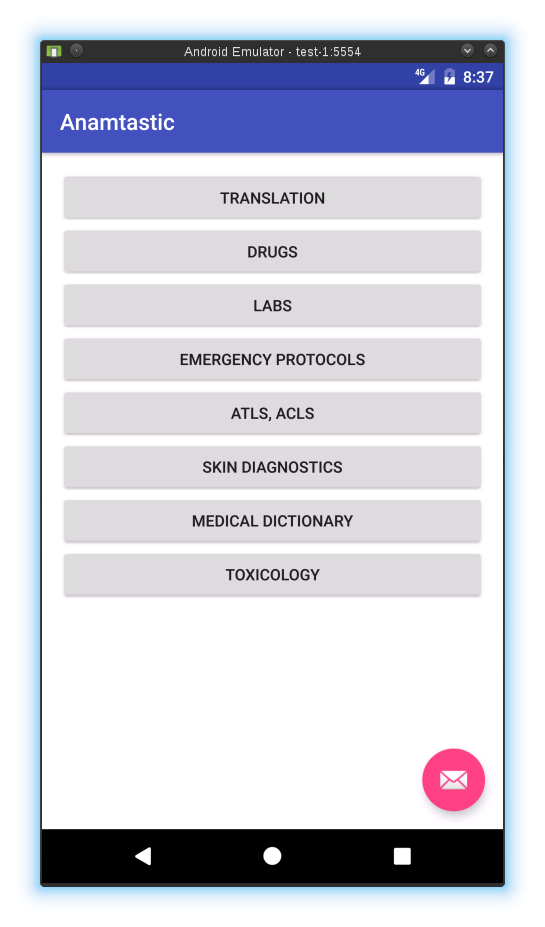
\includegraphics[width=3.6cm]{./presentation-images/module-selection-menu.png}
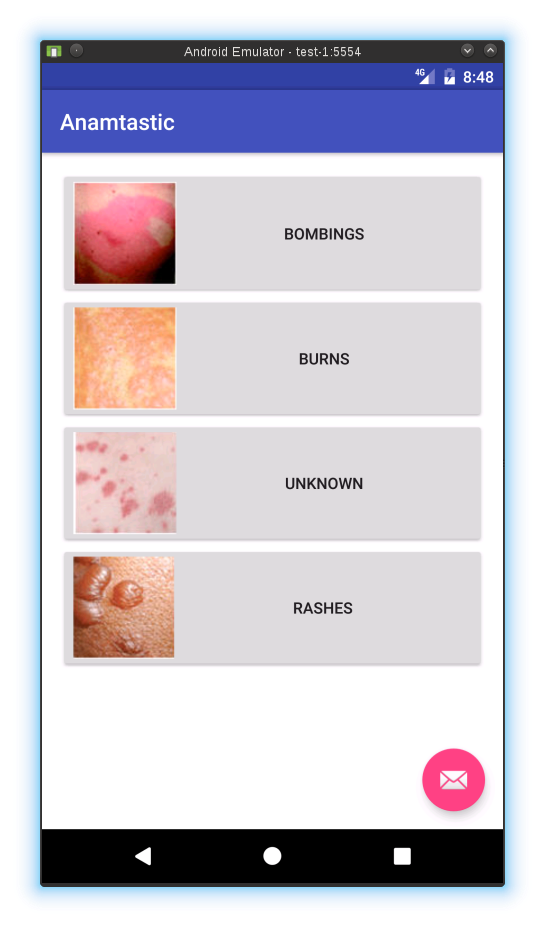
\includegraphics[width=3.6cm]{./presentation-images/skin-diagnostic-menu.png}
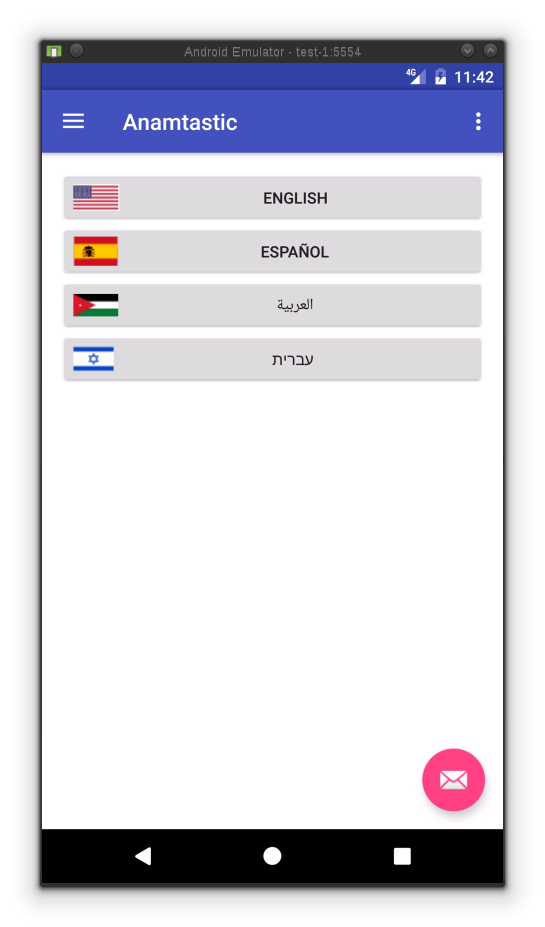
\includegraphics[width=3.6cm]{./presentation-images/language-select-menu.png}
\end{frame}

\subsection{Team}
\label{sec-1-7}
\begin{frame}[label=sec-1-7-1]{Team}
\begin{itemize}
\item Dr. Candace Makeda Moore, MD; (emergency doc, photographer, founder)
\item Dr. Jeremy Rutman, PhD, (patent attorney, computer programmer/image
processing, physicist)
\item Mike Green, MS (biologist, computer programmer)
\item Hagar Shilo, BA (front end developer, linguist)
\end{itemize}
\end{frame}

\subsection{Accomplishments}
\label{sec-1-8}
\begin{frame}[label=sec-1-8-1]{Accomplishments}
\begin{itemize}
\item Built website
\item Development of translation module underway, prototype/demo to be
completed on December 24$^{\text{th}}$, internal documents with algorithm and
design specifics currently in company dropbox
\item Collaboration with Trendiguru vis a vis Dr. Rutman to receive
algorithms for machine based 3D object recognition
\end{itemize}
\end{frame}

\subsection{The Real Plan}
\label{sec-1-9}
\begin{frame}[label=sec-1-9-1]{The Real Plan}
\begin{itemize}
\item As new modules are developed, starting with translation module
\item Try to sell modules to rivals i.e. PEPID, Epocrates, etc.
\item Try to push national acquisitions due to legal noncompliance
(providing care in patient's language mandated in some countries)
\item Business-wise we may be beat to market on some modules, but each can
be unpacked and sold once developed
\end{itemize}
\end{frame}
% Emacs 26.0.50.1 (Org mode 8.2.10)
\end{document}
